\documentclass[tikz, border=10pt]{standalone}
\usepackage[utf8]{inputenc}
\usepackage{tikz}
\usetikzlibrary{shapes.geometric, arrows.meta, positioning, calc}
\usepackage{amssymb} % For \mathbb

% Define custom colors from the SVG
\definecolor{boxFill}{HTML}{F2F7FF}
\definecolor{boxStroke}{HTML}{3366CC}
\definecolor{procFill}{HTML}{E8FFF2}
\definecolor{procStroke}{HTML}{33AA55}
\definecolor{lossFill}{HTML}{FFF2E6}
\definecolor{lossStroke}{HTML}{FF9933}

\begin{document}

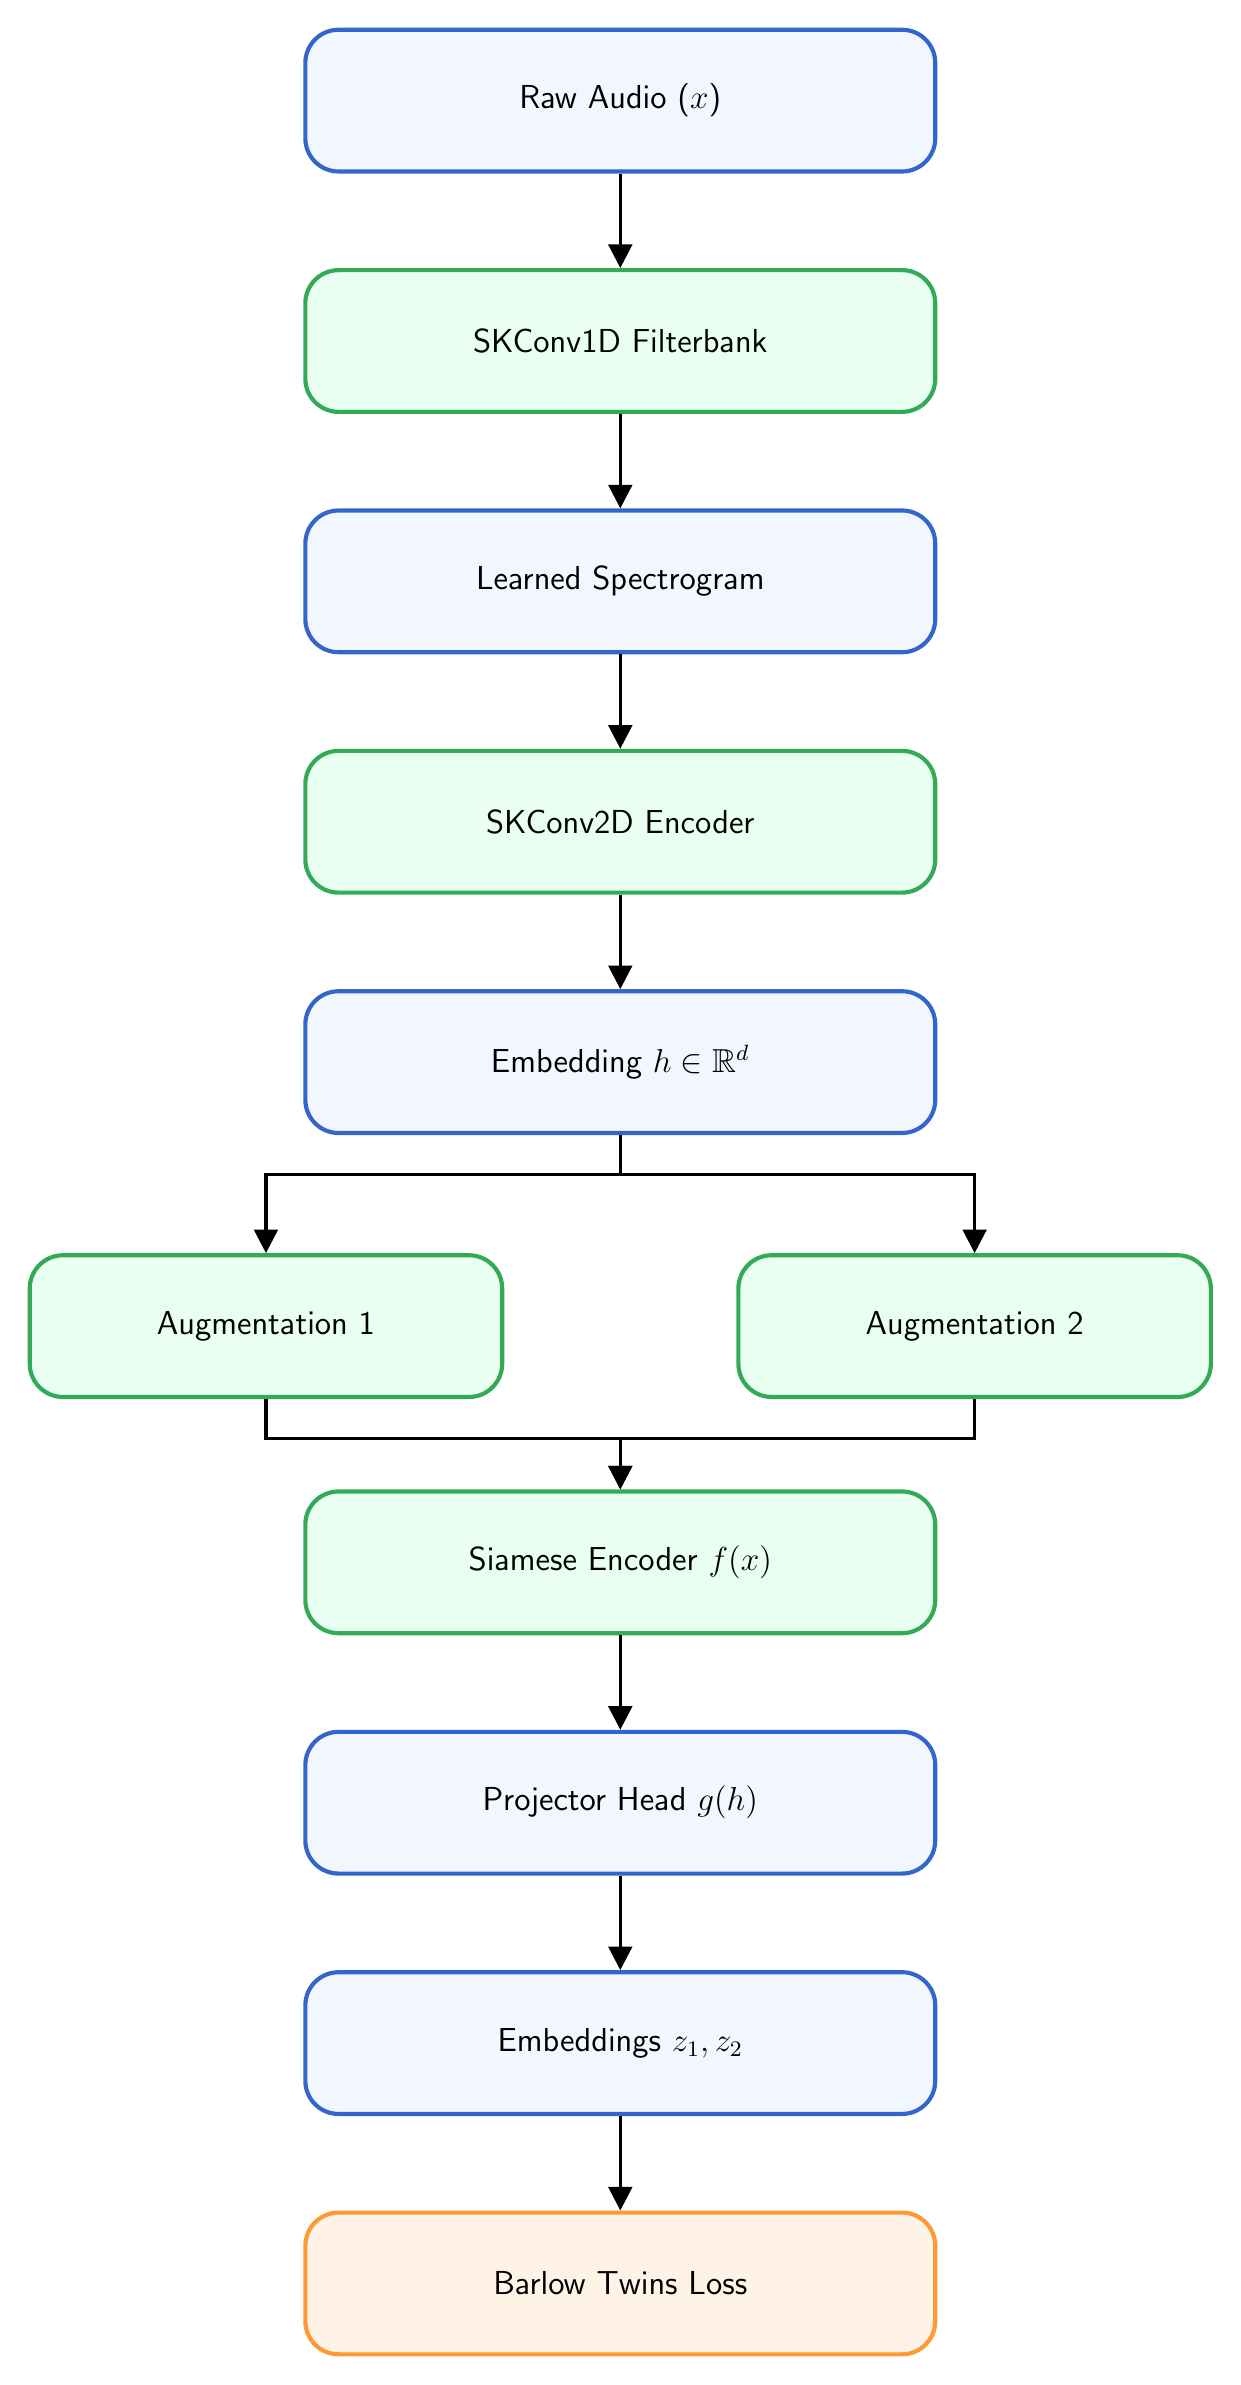
\begin{tikzpicture}[
    % Global Styles
    node distance=1.2cm,
    font=\sffamily\large,
    line width=1.5pt,
    % Node Styles matching SVG classes
    box/.style={
        rectangle, 
        rounded corners=12pt, 
        draw=boxStroke, 
        fill=boxFill, 
        align=center, 
        minimum width=8cm, 
        minimum height=1.8cm,
        inner sep=10pt
    },
    proc/.style={
        rectangle, 
        rounded corners=12pt, 
        draw=procStroke, 
        fill=procFill, 
        align=center, 
        minimum width=8cm, 
        minimum height=1.8cm,
        inner sep=10pt
    },
    loss/.style={
        rectangle, 
        rounded corners=12pt, 
        draw=lossStroke, 
        fill=lossFill, 
        align=center, 
        minimum width=8cm, 
        minimum height=1.8cm,
        inner sep=10pt
    },
    % Arrow Style
    arrow/.style={
        -{Triangle[length=3mm, width=3mm]}, 
        draw=black, 
        line width=1.2pt
    }
]

    % --- Nodes ---

    % 1. Raw Audio
    \node[box] (audio) {Raw Audio ($x$)};

    % 2. SKConv1D
    \node[proc, below=of audio] (filter) {SKConv1D Filterbank};

    % 3. Learned Spectrogram
    \node[box, below=of filter] (spec) {Learned Spectrogram};

    % 4. SKConv2D
    \node[proc, below=of spec] (enc2d) {SKConv2D Encoder};

    % 5. Embedding
    \node[box, below=of enc2d] (emb) {Embedding $h \in \mathbb{R}^d$};

    % 6. Augmentations (Split Branch)
    % We position these relative to the Embedding node, shifted left/right
    \node[proc, below=1.5cm of emb, xshift=-4.5cm, minimum width=6cm] (aug1) {Augmentation 1};
    \node[proc, below=1.5cm of emb, xshift=4.5cm, minimum width=6cm] (aug2) {Augmentation 2};

    % 7. Siamese Encoder (Merge Branch)
    % Positioned below the midpoint of the augmentations
    \node[proc, below=4.5cm of emb] (siam) {Siamese Encoder $f(x)$};

    % 8. Projector Head
    \node[box, below=of siam] (proj) {Projector Head $g(h)$};

    % 9. Embeddings z1, z2
    \node[box, below=of proj] (z) {Embeddings $z_1, z_2$};

    % 10. Loss
    \node[loss, below=of z] (loss) {Barlow Twins Loss};

    % --- Edges ---

    % Linear vertical connections
    \draw[arrow] (audio) -- (filter);
    \draw[arrow] (filter) -- (spec);
    \draw[arrow] (spec) -- (enc2d);
    \draw[arrow] (enc2d) -- (emb);

    % Split connections (Embedding -> Augmentations)
    \draw[arrow] (emb.south) -- ++(0,-0.5) -| (aug1.north);
    \draw[arrow] (emb.south) -- ++(0,-0.5) -| (aug2.north);

    % Merge connections (Augmentations -> Siamese)
    \draw[arrow] (aug1.south) -- ++(0,-0.5) -| (siam.north);
    \draw[arrow] (aug2.south) -- ++(0,-0.5) -| (siam.north);

    % Lower vertical connections
    \draw[arrow] (siam) -- (proj);
    \draw[arrow] (proj) -- (z);
    \draw[arrow] (z) -- (loss);

\end{tikzpicture}

\end{document}